%!TEX TS-program = xelatex
\documentclass[12pt, a4paper, oneside]{article}

\usepackage{amsmath,amsfonts,amssymb,amsthm,mathtools}  % пакеты для математики

\usepackage[utf8]{inputenc} % задание utf8 кодировки исходного tex файла
\usepackage[british,russian]{babel} % выбор языка для документа
\usepackage[X2,T2A]{fontenc}        % кодировка

\usepackage{fontspec}         % пакет для подгрузки шрифтов
\setmainfont{Helvetica}   % задаёт основной шрифт документа

% why do we need \newfontfamily:
% http://tex.stackexchange.com/questions/91507/
\newfontfamily{\cyrillicfonttt}{Helvetica}
\newfontfamily{\cyrillicfont}{Helvetica}
\newfontfamily{\cyrillicfontsf}{Helvetica}

\usepackage{unicode-math}     % пакет для установки математического шрифта
\setmathfont{Neo Euler}      % шрифт для математики
% \setmathfont[math-style=ISO]{Asana Math}
% Можно делать смену начертания с помощью разных стилей

% Конкретный символ из конкретного шрифта
% \setmathfont[range=\int]{Neo Euler}

%%%%%%%%%% Работа с картинками %%%%%%%%%
\usepackage{graphicx}                  % Для вставки рисунков
\usepackage{graphics}
\graphicspath{{images/}{pictures/}}    % можно указать папки с картинками
\usepackage{wrapfig}                   % Обтекание рисунков и таблиц текстом

%%%%%%%%%%%%%%%%%%%%%%%% Графики и рисование %%%%%%%%%%%%%%%%%%%%%%%%%%%%%%%%%
\usepackage{tikz, pgfplots}  % язык для рисования графики из latex'a

%%%%%%%%%% Гиперссылки %%%%%%%%%%
\usepackage{xcolor}              % разные цвета

\usepackage{hyperref}
\hypersetup{
	unicode=true,           % позволяет использовать юникодные символы
	colorlinks=true,       	% true - цветные ссылки, false - ссылки в рамках
	urlcolor=blue,          % цвет ссылки на url
	linkcolor=red,          % внутренние ссылки
	citecolor=green,        % на библиографию
	pdfnewwindow=true,      % при щелчке в pdf на ссылку откроется новый pdf
	breaklinks              % если ссылка не умещается в одну строку, разбивать ли ее на две части?
}


\usepackage{todonotes} % для вставки в документ заметок о том, что осталось сделать
% \todo{Здесь надо коэффициенты исправить}
% \missingfigure{Здесь будет Последний день Помпеи}
% \listoftodos --- печатает все поставленные \todo'шки

\usepackage{enumitem} % дополнительные плюшки для списков
%  например \begin{enumerate}[resume] позволяет продолжить нумерацию в новом списке

\usepackage[paper=a4paper, top=20mm, bottom=15mm,left=20mm,right=15mm]{geometry}
\usepackage{indentfirst}       % установка отступа в первом абзаце главы

\usepackage{setspace}
\setstretch{1.15}  % Межстрочный интервал
\setlength{\parskip}{4mm}   % Расстояние между абзацами
% Разные длины в латехе https://en.wikibooks.org/wiki/LaTeX/Lengths


\usepackage{xcolor} % Enabling mixing colors and color's call by 'svgnames'

\definecolor{MyColor1}{rgb}{0.2,0.4,0.6} %mix personal color
\newcommand{\textb}{\color{Black} \usefont{OT1}{lmss}{m}{n}}
\newcommand{\blue}{\color{MyColor1} \usefont{OT1}{lmss}{m}{n}}
\newcommand{\blueb}{\color{MyColor1} \usefont{OT1}{lmss}{b}{n}}
\newcommand{\red}{\color{LightCoral} \usefont{OT1}{lmss}{m}{n}}
\newcommand{\green}{\color{Turquoise} \usefont{OT1}{lmss}{m}{n}}

\usepackage{titlesec}
\usepackage{sectsty}
%%%%%%%%%%%%%%%%%%%%%%%%
%set section/subsections HEADINGS font and color
\sectionfont{\color{MyColor1}}  % sets colour of sections
\subsectionfont{\color{MyColor1}}  % sets colour of sections

%set section enumerator to arabic number (see footnotes markings alternatives)
\renewcommand\thesection{\arabic{section}.} %define sections numbering
\renewcommand\thesubsection{\thesection\arabic{subsection}} %subsec.num.

%define new section style
\newcommand{\mysection}{
	\titleformat{\section} [runin] {\usefont{OT1}{lmss}{b}{n}\color{MyColor1}} 
	{\thesection} {3pt} {} } 


%	CAPTIONS
\usepackage{caption}
\usepackage{subcaption}
%%%%%%%%%%%%%%%%%%%%%%%%
\captionsetup[figure]{labelfont={color=Turquoise}}

\usepackage[normalem]{ulem}  % для зачекивания текста

\pagestyle{empty}

\begin{document}
	
	
	\subsection*{[5]   Упражнение 1 (Пожалуй, самый сложный пакет в вашей жизни ) }
	
	Суть этого упражнения сводится к тому, что вы должны заставить работать пакет minted.  Этот пакет вы в будущем будете использовать для оформления кода.  Напоминаю, что этот пакет написан на Python. Это означает, что для использования minted должен быть установлен Python. \textbf{Следуя инструкции ниже, установите minted.} 
	
	\textbf{Windows:}
	
	\begin{enumerate}
		\item Устанавливаем на компьютер Python. Лучше всего поставить дистрибутив, который называется \href{https://docs.continuum.io/anaconda/install}{Anaconda.} Этот дистрибутив включает в себя все основные пакеты, которые необходимы для работы с питоном. 
		
		\item Открываем консоль. Для этого жмём \texttt{win+R}, вводим в открывшемся окне \texttt{cmd}, жмём \texttt{enter}.  Открывается командная строка. 
		
		\item Прописываем в командной строке \texttt{pip install Pygments}
		
		\item Команда выше установила на наш компьютер питоновский пакет, который будет раскрашивать код в \LaTeX{}. Теперь нужно настроить texstudio. Заходим в настройки и там прописываем в графе  XeLatex: \newline  \texttt{Xelatex -shell-escape -synctex=1 -interaction=nonstopmode \%.tex`}
		
		\item Эта команда подключает к теху внешние пакеты. В нашем случае это Pygments. 
	\end{enumerate} 
	
	
	\textbf{Linux (Ubuntu 16):}
	
	\begin{enumerate}
		\item Если честно, то в Anaconda много бесполезного хлама. И лучше приручать змей вручную. Но не на Windows. Жмём \texttt{ctrl+alt+T}, открывается терминал. 
		\item Убеждаемся, что установлен Python, вбивая в терминале \texttt{python --version}, а он установлен, потому что половина системы на нём написана.
		\item Убеждаемся, что установлен pip, вбивая  \texttt{pip --version}. Если он не установлен, то ставим его!  \texttt{sudo apt-get install python-pip}.
		\item Устанавливаем наш пакет  \texttt{sudo pip install Pygments}
		\item Заходим в настройки texmaker и там прописываем в графе  XeLatex:  \newline \texttt{Xelatex -shell-escape -synctex=1 -interaction=nonstopmode \%.tex`}
	\end{enumerate} 
	
	\textbf{Mac:}
	
	\begin{enumerate}
		\item Оказывается, у вас на macOS уже стоит python. Еси открыть терминал, то можно убедиться в этом, прописав \texttt{python --version}
		\item Убеждаемся, что установлен pip, вбивая  \texttt{pip --version}. Если он не установлен, то ставим его!  
		\item Устанавливаем наш пакет  \texttt{sudo pip install Pygments}
		\item  Готово! Теперь, если вы спросите \texttt{which pygmentize}, то  ответ должен быть такой  \texttt{pygmentize is /usr/local/bin/pygmentize}
		\item Теперь можно запускать техмейкер/техстудио/техпад, подключать minted и, если вы не забыли в настройках  в графе  XeLatex:  подписать  \texttt{Xelatex -shell-escape -synctex=1 -interaction=nonstopmode \%.tex`}, то всё должно работать.
	\end{enumerate} 
	
	
	После всех этих действий вы должны почувствовать себя супермега программистом. Дело осталось за малым. Создаём теховский документ, подключаем пакет minted и используем окружение minted. Вы ещё не забыли, что задание состояло в том, что нужно оформить какой-нибудь кусочек своего кода с помощью minted? Именно за оформление любого кода вы и получите свои честно заработанные баллы. 
	
	
	
	
	
	
	\section*{Задание 5  (20 баллов)  }
	
	\textbf{Это задание не является обязательным!}   Не забывай, где находится  \href{https://fulyankin.github.io/LaTeX/}{страничку курса} с кучей шпаргалок! Как правильно себя вести — вы уже знаете. Вот вам \href{https://docs.google.com/forms/d/e/1FAIpQLSe11kxKVfv07iCL1E9yNX7ll9swKImiVwRr1H70lslGzInRSg/viewform}{уютная гугл-форма.}   Не стеснятесь просить о помощи, если она вам необходима. \textbf{Дедлайн:  } 
	
	\todo[inline]{Дедлайн до окончания курса.}

\subsection*{[15]  Упражнение 1  (Свои собственные)}

Создайте следующие команды и продемонстрируйте как они работают. Если вы не приводите пример работы команды, то вы не получаете за неё баллы.

\begin{itemize}
	\item[$(1)$] Создайте такие математический операторы, как \verb|Var| и \verb|Cov|.
	\item[$(1)$] Вы всё время по ходу текста должны писать \verb|\sigma|-алгебра. Напишите команду, которая позволит делать это без перехода в математический режим. Например,  \verb|\s|-алгебра.
	\item[$(1)$] Написать команду, которая будет выводить $x_1 \ldots x_n$
	\item[$(2)$] Усовершенствовать предыдущую команду. Она должна быть от двух аргументов и при запросе \verb|\com{a}{z}, \com{1}{6}| и \verb|\com{(a,b)}{(c,d)}| выдавать соответственно:  $x_a \ldots x_z$, 
	$x_1 \ldots x_6$ и   $x\_{(a,b)} \ldots x\_{(c,d)}$
	\item[$(2)$] Сделать так, чтобы в itemize каждый новый пункт шёл после синей точки.
	
		\todo[inline]{Пример.}
	
	
	
	\item[$(2)$] Вспомните проблемы с самой первой пары. Мы писали внутри текста \verb|\lim_{x \to 0} \frac{\sin{x}}{x}| и получали не очень привычную для нашего восприятия формулу. После мы добавляли \verb|\limits| и формула становилась более привычной. Определите команду \verb|\llim| так, чтобы внутри текста всегда получать формулу в привычном виде.
	\item[$(2)$] Сделайте нумерацию рисунков в документе в следующем формате: "номер секции: номер рисунка". Обязательно приложите к файлу рисунок, который вы будете использовать для демонстрации своих достижений.
	\item[$(2)$] Пусть все формулы нумеруются вот так: 
	
			\todo[inline]{КАК.}
	
	\item[$(2)$] Написать команду или окружение с несколькими аргументами. Текст внутри него должен переворачиваться вверх ногами и (или) переворачиваться зеркально. При её написании можно использовать etoolbox. А можно не использовать. А можно использовать, но как бы чуть-чуть...
	\item[$(5)$] Придумайте команду, которая здорово упростит жизнь всему человечеству! Баллы выдаём за каждую. 
\end{itemize}

\subsection*{[15]  Упражнение 2  (Cowsay)}

Cowsay — это настраиваемая говорящая и думающая корова! Эта\href{http://citkit.ru/articles/679/}{великая программа} была когда-то написана на Perl и с тех пор не может покинуть многие великие умы.

Если вы используете Linux, то вы можете поставить cowsay, прописав \texttt{sudo apt-get install cowsay}. После попробуйте ввести \texttt{cowsay Hello, World!}. Если у вас Mac, вы можете сделать всё то же самое через `brew`. Если у вас Windows, то побаловаться с коровой будет не очень просто. Не забудьте вернуться назад, в наш бренный мир, после экстаза, который вы испытаете!

\begin{center}
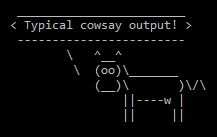
\includegraphics[scale=1]{Cowsay_Typical_Output.png}
\end{center}

Создайте в LaTeX своё окружение, которое будет работать по аналогии с cowsay. Нарисуйте все необходимые для него кусочки в Tikz. Можете использовать для этого Geogebra или уже готовые заготовки, которые вы найдёте на просторах интернета. Оригинальные ходы будут щедро поощрены.





\subsection*{[0 - 100 ]  Упражнение 3  (Наклеечи)}

Каждые полгода в Москве проходит \href{http://datafest.ru/}{Датафест.} Одно из самых крупных собраний датамайнеров. На каждый датафест печатается партия отличных наклеек! Главная особенность этих наклеек состоит в том, что их хотят все.

\begin{center}
	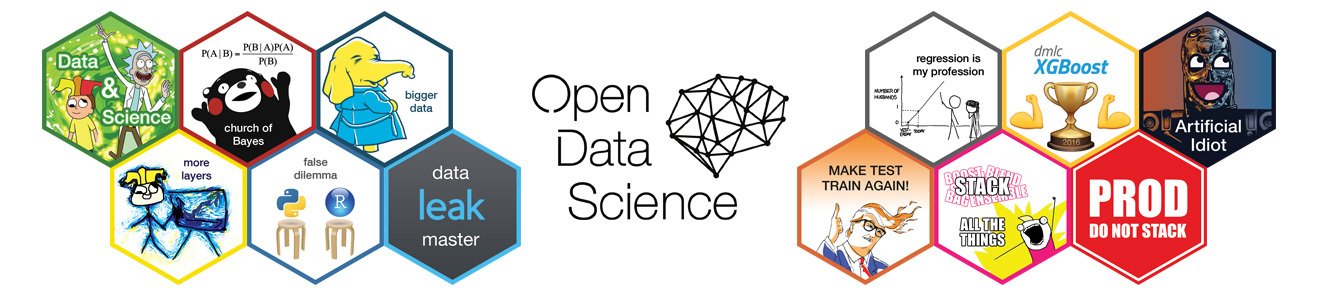
\includegraphics[scale=0.35]{DF.jpg}
\end{center}

\todo[inline]{Переписать на актуальную инфу}

Новый датафест уже был 11 февраля в небоскрёбе Mail на станции метро Аэропорт. Следующий будет осенью в здании Yandex на Парке Культуры. Непременно посетите его... Нарисуйте свою наклейку, используя средства Tikz. Идеология наклеек следующая: на наклейке должен быть либо общеизвестный символ, либо тонкая профессиональная шутка. Например, если вы рисуете макроэкономическую наклеечку, то любой другой случайно заметивший её макроэкономист, например работающий в ЦБ, должен понять нарисованную шутку и захотеть такую наклейку себе. Более того, вы сами должны хотеть прилепить такую наклейку на крышку своего ноута или на другое видное место.

На рисование наклеек отводится три недели (крайний срок - 11 часов утра 22 марта). По истечению этого срока самые интересные наклейки будут выставлены на суд публики. Лучшие из них будут напечатаны и растиражированы на 9 неделе! Не переборщите со сложностью наклеек. Люди должны понимать, что на них нарисовано...


\end{document}